% Imported from algorithms/long-video/README.md
\chapter{长上下文与缓存条件}\label{seedance-m06}
\moduleinfo{M06}{基础方法与机制解释}{\hyperref[src-long-context-tuning]{\texttt{long-context-tuning}}、\hyperref[src-longlive]{\texttt{longlive}}、\hyperref[src-seedance-1.0]{\texttt{seedance-1.0}}、\hyperref[src-longlive-code]{\texttt{longlive-code}}}

短片采样之后再扩展时间：这里先说明长上下文与固定历史各需要怎样的信息依赖。

视频继续变长，原来的局部生成问题就变成了带历史的生成。前面的人物、道具和动作状态，会约束下一段应该出现什么。若模型只在短片上训练，推理时却不断读取自己刚生成的历史，误差会改变后续条件，再一段段传下去。身份漂移、背景突变和剧情遗忘都可以沿这条关系分析。

\section{先区分三种长视频}\label{seedance-m06-ux5148ux533aux5206ux4e09ux79cdux957fux89c6ux9891}

先分任务。多镜头可以切镜，但要共享角色、环境和事件；长单镜头还要求运动与相机空间连续；交互续写则把已完成历史固定，再接受新提示。三者都可能很长，所需上下文却不同，所以不能只用一分钟总时长来判断是否解决了同一个问题。

描述也随之分成两层：全局写角色、环境和故事，镜头内写局部动作、景别和运镜。这样哪些信息应延续、哪些信息本镜头应变化，就不必全部挤在一段没有归属的文字里。

\section{多镜头为什么适合异步噪声}\label{seedance-m06-ux591aux955cux5934ux4e3aux4ec0ux4e48ux9002ux5408ux5f02ux6b65ux566aux58f0}

普通联合去噪可以让所有镜头处在同一个噪声时间；异步训练则给每个镜头独立的 \(t_s\)。较干净的镜头提供身份和环境线索，较噪的镜头学习利用这些线索生成。

这种任务需要逐镜头时间条件，不能只把输入噪声改成不同强度，却仍向网络提供同一个时间。训练完成后，既可以共同生成一组镜头，也可以固定已有镜头，再生成后续镜头。

双向注意力允许镜头相互约束；上下文因果注意力则规定镜头内双向、镜头间只能读取过去与当前。先训练双向模型、再做因果适配是一条可行路线，但不是所有模型都必须遵守的固定顺序。

\section{因果 mask 为什么还不足以支持缓存}\label{seedance-m06-ux56e0ux679c-mask-ux4e3aux4ec0ux4e48ux8fd8ux4e0dux8db3ux4ee5ux652fux6301ux7f13ux5b58}

缓存究竟缓存了什么？某一层的 key/value，是由历史潜变量和上游隐藏状态计算的，也依赖提示、参考、噪声时间、位置、mask 与权重。只有这些依赖没有变，读取旧值才等价于再算一次。先明确这个条件，再讨论缓存能省多少。

普通扩散每一步都改整个带噪序列 \(z_t\)，历史特征也随之改变。即使加了因果 mask，只要历史内容或它使用的噪声时间还在变，上一去噪步的 K/V 就不是当前这一步的 K/V。因果可见性与跨步不变性，在这里是两个不同条件。

所以精确缓存通常要给历史一个固定的条件身份：内容、噪声水平及条件化方式都不再随活动块改变。当前块仍在去噪，每一步照常算自己的 Q、K、V，再去读这段固定历史。这才把可复用部分与变化部分接起来。

\section{缓存究竟省掉多少计算}\label{seedance-m06-ux7f13ux5b58ux7a76ux7adfux7701ux6389ux591aux5c11ux8ba1ux7b97}

设视频有 \(S\) 个块，每块 \(n\) 个 token。如果生成第 \(i\) 块时重新处理全部前缀，投影和 FFN 累计处理的 token 数为：

\[
n\sum_{i=1}^{S}i=O(nS^2).
\]

若每次还对整个前缀做完整注意力，累计交互规模为：

\[
n^2\sum_{i=1}^{S}i^2=O(n^2S^3).
\]

缓存固定历史后，可以省掉重复的历史投影和前馈计算，但第 \(i\) 块仍要查询前面约 \(i\) 个块，累计 attention 成本约为：

\[
n^2\sum_{i=1}^{S}i=O(n^2S^2).
\]

只有进一步把可读历史限制为固定的 \(W\) 个块，才会接近 \(O(Sn^2W)\)。因此，``使用 cache''与``总计算随时长线性增长''不是同一个结论。以上省略了层数与每块去噪步数，实际实现还需乘回这些因素。

\section{流式训练怎样缩小训练与推理差距}\label{seedance-m06-ux6d41ux5f0fux8badux7ec3ux600eux6837ux7f29ux5c0fux8badux7ec3ux4e0eux63a8ux7406ux5deeux8ddd}

训练与这种推理怎样接近？可以让模型逐渐读取自己产生的历史，而不只看完美真实历史。每次只对当前短片段反传，历史停止梯度，再逐步延长序列。这样当前目标面对的条件更接近续写时真正遇到的状态。

\begin{figure}
\centering
\pandocbounded{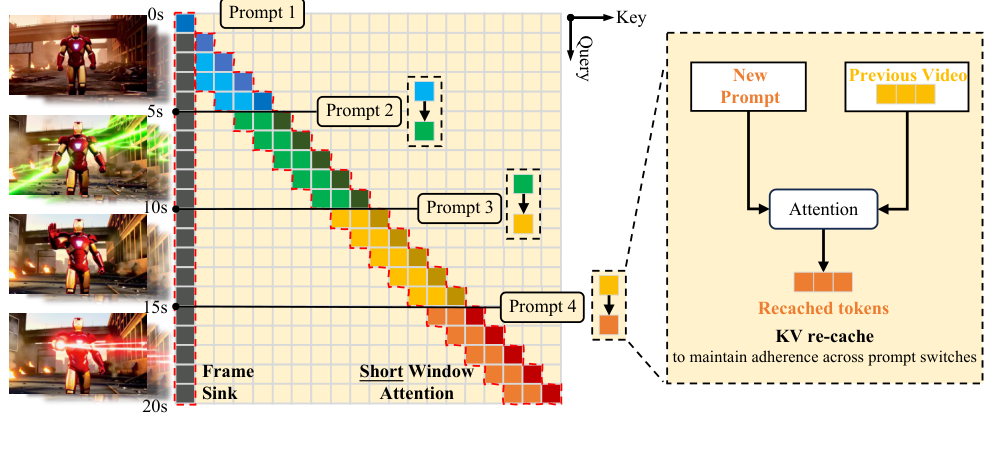
\includegraphics[keepaspectratio,alt={短窗口、历史锚点与提示切换时的缓存刷新 （论文示意，来源：longlive）}]{assets/seedance/figures/streaming-cache.png}}
\caption{短窗口、历史锚点与提示切换时的缓存刷新 （论文示意，来源：longlive）}
\end{figure}

图中短窗口控制近期历史的计算量，早期锚点提供身份和场景线索；提示变化后，则用历史画面与新提示重新建立缓存。它们分别作用于成本、保持和条件更新，需要与同一套训练及推理依赖对应。

但早期锚点也不能代替全部事件状态。人物后来拿起钥匙，开头没有这件事，继续读开头仍然不知道钥匙现在在哪里。于是还需要近期事件或主体状态的记忆，窗口大小和剧情记忆不能当成同一个参数。

\section{怎样验证缓存和长程记忆}\label{seedance-m06-ux600eux6837ux9a8cux8bc1ux7f13ux5b58ux548cux957fux7a0bux8bb0ux5fc6}

先以不使用缓存的完整重算结果为基线，在相同噪声下逐层比较输出；再分别改变提示、参考、历史和时间条件，确认系统会使相应缓存失效。修改过去片段时，因果模型的该片段及后续缓存通常需要刷新，双向场景模型甚至可能影响整场景。

长程效果再按时间分段看。可将生成长度扩到训练长度的两倍、四倍，记录各段身份、道具、背景与动作错误，同时单独观察新提示多久生效。只给整段一个平均分，后半段崩坏可能被前半段掩盖。缓存与这些保持问题都确认后，再继续调窗口、精度和吞吐。

\section{从极简代码到真实实现}\label{seedance-m06-ux4eceux6781ux7b80ux4ee3ux7801ux5230ux771fux5b9eux5b9eux73b0}

缓存首先是依赖版本问题。提示、历史、噪声策略或模型改变时，旧状态就不能继续当成相同条件：

\begin{verbatim}
key = hash_of(model, prompt, references, history, noise_policy)
if key != previous_key:
    cached_layers.clear()
\end{verbatim}

\hyperref[code-cache-context]{cache\_context.py} 只说明失效机制，没有实现完整自回归 attention。真实的缓存写入、当前块去噪和窗口读取，直接看 \href{https://github.com/NVlabs/LongLive/blob/31c70d9071cd7851d82939806dc9fac645fcabe5/LongLive1.0/pipeline/causal_inference.py}{LongLive1.0 因果推理} 与 \href{https://github.com/NVlabs/LongLive/blob/31c70d9071cd7851d82939806dc9fac645fcabe5/LongLive1.0/wan/modules/causal_model.py}{CausalWanSelfAttention}。普通双向模型无法只靠添加这个字典获得相同能力。
